\chapter{Introduction}
\todo{Font 12 - blås opp tekstene/mer tekst på sidene(Bacheor thisis?)}
\section{Project group}
The bachelor group consists of the following four IT students:
\begin{itemize}
    \item Andreas Harnes. 
    Computer Science student with interests in networking and programming.
    \item Celina Marie Kristiansen.
    Computer Science student with experience in databases and big data.
    She has previously been deployed at Logiq where she used Databricks to process data.
    \item Magnus Klerck.
    Information systems student with background as a computer electrician where he worked with IT maintenance and hardware repair.
    He also has an interest in cybersecurity.
    \item Morten Offerdal Kvigne.
    Computer Science student with interests in programming and data security.
\end{itemize}
Celina M. Kristiansen, Magnus Klerck and Morten Offerdal Kvigne have previously been working on projects together.
The three had effective collaborations in their former projects which is reflected in the results they produced.
Due to the effective collaboration the three of them decided to form this bachelor group.

Magnus and Morten had both previously worked with Andreas Harnes and they both believed him to be knowledgeable and as such he was brought in.

\section{Assignment provider}
\todo{Skriv først om HiØ, deretter MakerSpace}
\todo{Campus Halden, not in Halden(?)}
MakerSpace is a workspace at Østfold University College in Halden. 
The workspace acts as a playground for students and employees who like to use technology to create something \cite{what-is-makerspace}.
MakerSpace is operated by Michael Andersen Lundsveen and 4 student assistants but all students and employees at Østfold University College have access to the facility 24 hours, 7 days a week
\cite{what-is-makerspace}.
Østfold University College describes the drive behind MakerSpace as:

\begin{displayquote}
The purpose of Makerspace is to offer students a physical space and an engaging environment with the aim to learn something new by encouraging curiosity and eagerness \cite{what-is-makerspace}.
\end{displayquote}
In addition MakerSpace also acts as an area for lectures, courses and experiments.
They also hold basic programming courses for children during the summer.

MakerSpace is equipped with various equipment related to several fields.
Some of the equipment MakerSpace offers is 3D printers, which can be used to print out different figures and shapes in plastic from a 3D model. Soldering irons for making circuits and soldering components, computers with VR headsets, lego robots and remote controlled drones as shown in figure \ref{fig:makerspace}. MakerSpace also has different tools like screwdrivers, workbenches, pliers, RJ45 crimpers to mention some.

Lastly MakerSpace allows students and employees at Østfold University College to borrow equipment.
Students and employees have to note down their name, their contact information and the item(s) they are lending in a book used to keep track of all borrowed equipment whenever they are borrowing equipment.

MakerSpace responsible Michael Andersen Lundsveen is the assignment provider for the project. 
Michael is the leader and principal engineer for MakerSpace Halden.
He oversees day to day operations and he ensures all equipment is in good condition.
Additionally he is responsible for the repairment or the purchase of new equipment should equipment be damaged or destroyed.
Michael also arranges courses for the MakerSpace employees allowing them to learn how to utilize new equipment, he arranges summer workshops for children during the summer vacations and he sponsors certain arrangements and events at Halden University College.

\begin{figure}
    \centering
    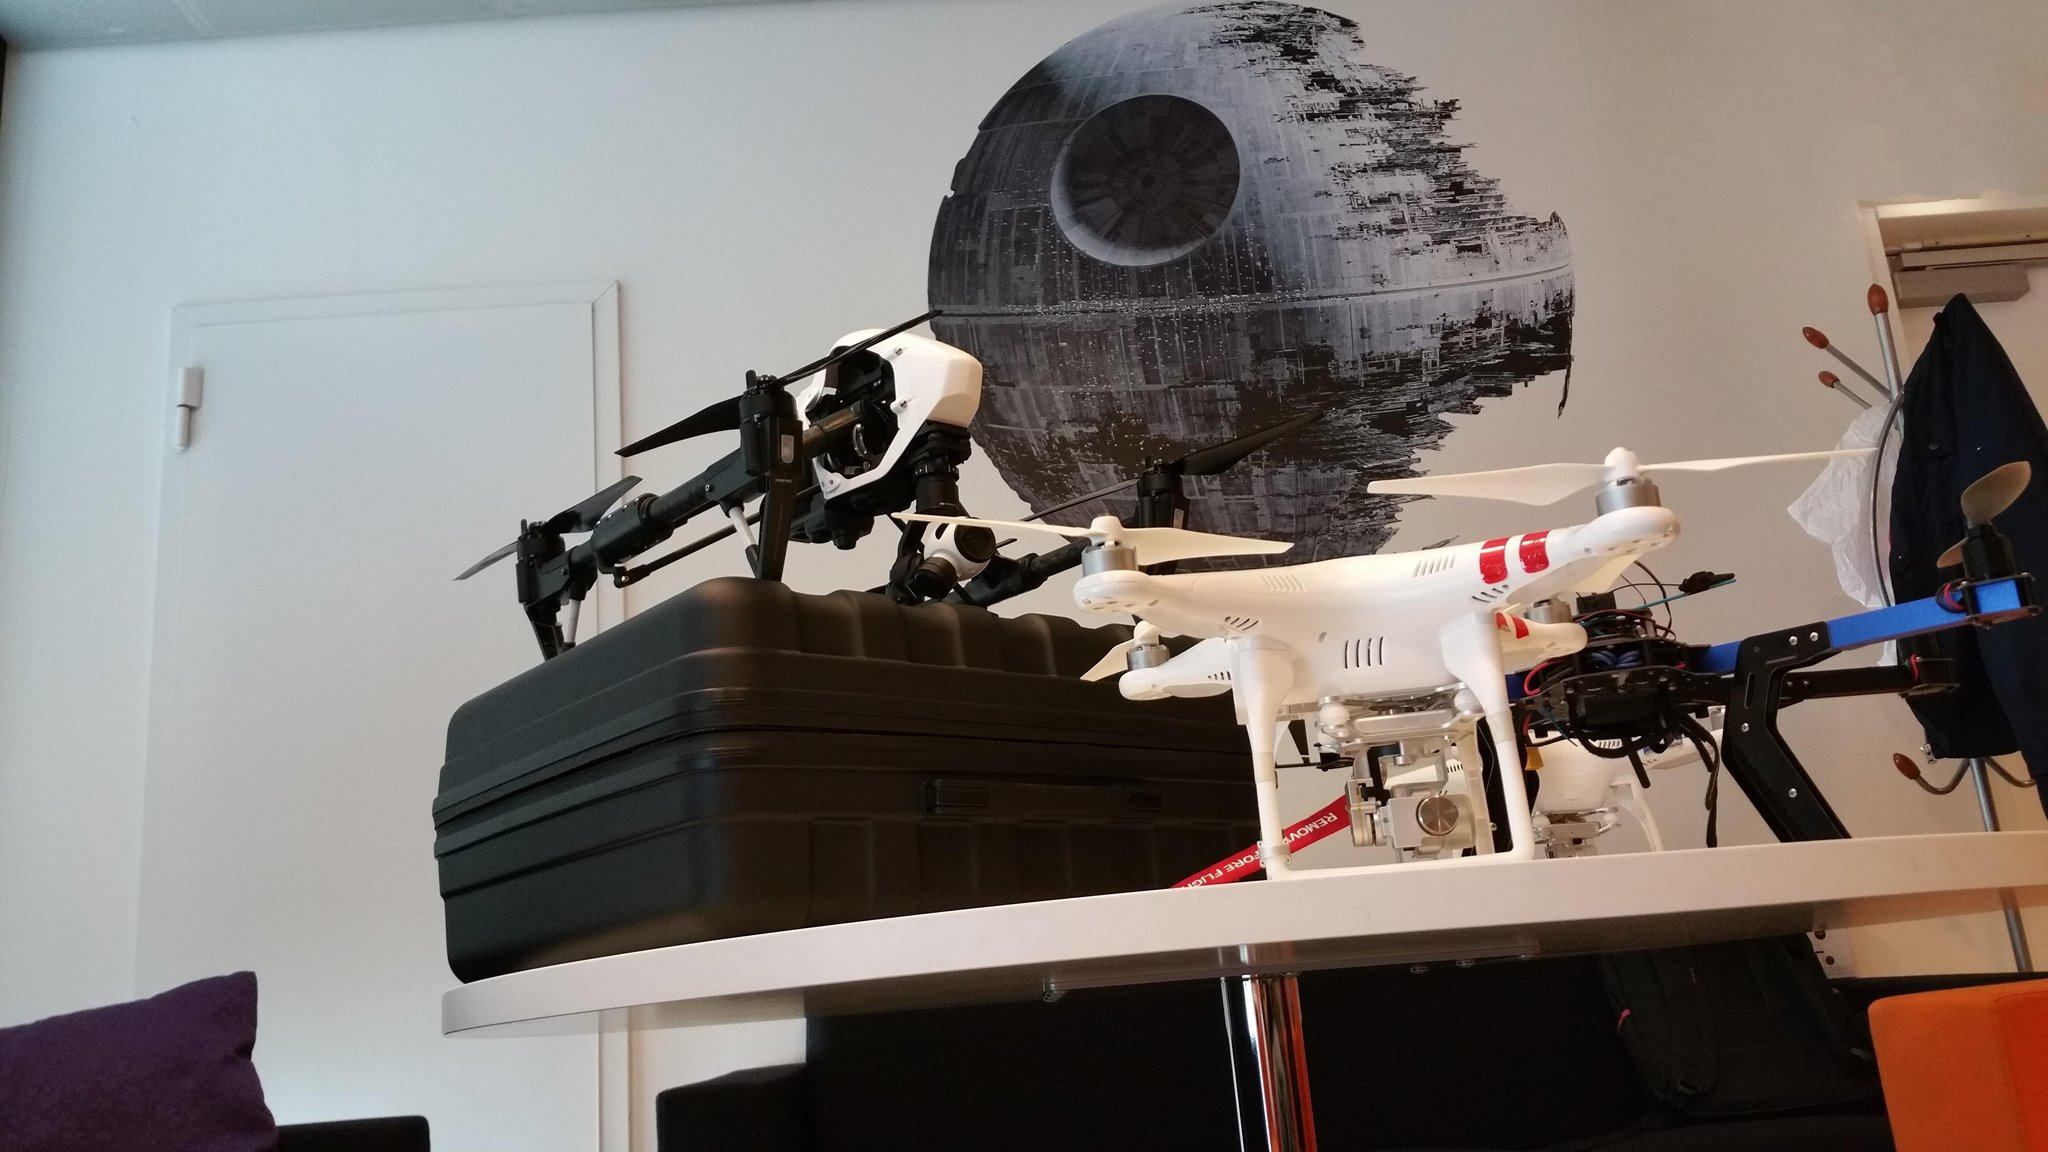
\includegraphics[width=115mm,scale=1]{images/makerspace.png}
    \caption{Remote controlled drone}
    \label{fig:makerspace}
\end{figure}

\section{The mission}
The background for the project is that MakerSpace currently does not have an overview of what equipment they have, or if the equipment is available and where the equipment is stored.
This is problematic for the employees at MakerSpace as they have no way of knowing whether the equipment is missing or if the equipment is damaged.
Even if an employee is made aware of missing or damaged equipment the employee currently has no way of notifying the other employees and as such the employee will have to manually contact the other employees in order to notify them which is cumbersome.

This is also problematic for the users of MakerSpace.
The users have to search through MakerSpace in its entirety in order to find a given piece of equipment.
They have no way of knowing whether the piece of equipment is damaged until they find it.
They also have no way of knowing whether MakerSpace has the piece of equipment or if another user is currently borrowing it.

Lastly the book used when borrowing equipment also proves problematic.
Anyone can inspect the contents of the book and as such the book does not respect the privacy of the users.
This is concerning should the book be stolen, because all the names and contact information of the users will be astray.
Finally the book is not protected in the event of a fire and all information would be lost.

In order to solve the issues outlined above the group intends to develop two modules.
The employees and users will interact with the modules using web pages.
The following two modules will be developed:
\begin{itemize}
    \item An inventory module allowing employees and users to view the equipment MakerSpace offers, the equipment's condition, where the equipment is stored and weather the equipment is available.
    The module will also allow employees to add, modify and delete equipment from the module.
    \item A lending module allowing employees and users to borrow equipment.
    When returning equipment the module also allows the employee or the user to report any damage that occurred whilst the equipment was being borrowed.
\end{itemize}

The modules will be extendable.
This allows future features to be incorporated into the modules without difficulties for future developers.

%What MakerSpace wants is a system that gives Michael and student assistants access to an overview of all the equipment and tools available in MakerSpace. This system must be modular so that it can be further developed later, and in addition to this a inventory system. They also want a lending module that makes it easier to register the lending of equipment and tools.

%What the group is planning to develop is a modular inventory system and a lending module by adopting technology that is in use today.

%\todo{TODO Alt under flyttes til metode}
%\textbf{Investigation:} The group have talked about some technology they could potentially use. Some of the technology the group have been thinking about is: Vue.js, Node.js and MongoDB. The group will do a investigation for each of those and find out if they fit the project or not. The group will also try and find other technologies that can be more applicable for the project.

%\textbf{Development:} The group will create a website that will offer a lending system of equipment that exists at MakerSpace and also make sure that the system can be further developed later on.

%In the development of the system, the group have made some bullet-points as an overview for the project. These are:
%\begin{enumerate}
%  \item Make the website that will be used for the system and make sure it follow the criteria for universal design.
%  \item Design a structure for the inventory storage.
%  \item Make a module for lending.
%  \item User test the system to find bugs.
%\end{enumerate}

\section{Purposes and delivery}
\subsection{Purposes}
%There are two reasons for the project.
%The first is to provide an overview of the equipment available at MakerSpace to the employees and users of MakerSpace.
%This is beneficial as the employees and users now no longer need to search through MakerSpace in its entirety to see if MakerSpace offers the equipment they seek.

%The second reason is to digitize the lending system MakerSpace currently has in place.
%This is beneficial because it is privacy respecting as only those with the necessary permissions can view the records of equipment currently being borrowed. 
%Additionally should equipment not be returned MakerSpace will know who is responsible.
%Lastly the records of borrowed equipment can be place on a backup - meaning the records of borrowed equipment are not lost in case of theft or in case of a fire.

\textbf{Main goal:} Make an inventory module which provides an overview of the equipment available at MakerSpace.

\textbf{Sub goal 1:} Make a lending module which digitizes the current lending system used at MakerSpace.

%The purposes with this project is to digitize the current lending system. This will make it easier to not only see what equipment that is available for lending but also what equipment that needs to be order more of. This is divided into a main goal and some sub-goal's.

%\textbf{Main goal:} Digitize current lending system and write the report.

%\textbf{Sub-goal 1:} Make a inventory structure with a lending module

%\textbf{Sub-goal 2:} Make sure that the website (e.g front-end, UI,UX) follow the criteria for universal design.

\subsection{Delivery}

Below are the deliveries the group will deliver during the project.

\begin{tabu} to 1.2\textwidth { | X[l] | X[c] | }
    \hline
    \textbf{Date} & \textbf{Delivery} \\
    \hline
    January 18 ,2019 & Pilot report \\
    \hline
    March 08, 2019 & First version of main document \\
    \hline
    April 23, 2019 & Second version of main document \\
    \hline
    April 26, 2019 & Product \\
    \hline
    May 16, 2019 & Finished version of main document \\
    \hline
    May 27, 2019 & Project poster \\
    \hline
   June 03, 2019 - June 05, 2019 & Presentation of the project \\
    \hline
\end{tabu}
    
\section{Method}
bla bla tekst om hvilke metoder vi velger å bruke etc...
\todo{Metode skal vise kva metode me skal bruke i research og utvikling}
\todo{Hvordan intervju folk? Skrive om spørreskjema. Hva gjør me med resultatet av spørreskjemaet?}
\todo{Hvordan skal me testa, kva testmetoder?}
\todo{Hvordan skal me søke informasjon? Skal me bruke agile metoder sammen med Michael elelr skal me berre få ein plan fra Michael også utvikle det? Me har ikkje valgt waterfall pga ..., derimot bruker me agile pga ... Ofte knyttat mot teorien på den}
\todo{Ang spørreskjema. Korleis skal me samle info, intevjue, sende spørreskjema, korleis skal me bearbeide det}

\subsection{Agile(?)}
\todo{Her starter Agile}The group has decided to use an agile model for the software development process.
The project is small in scale and is not tightly integrated with any other system.
This means the comprehensive documentation a waterfall model requires is not needed.
Additionally this means informal communications between group members work well as the group is co-located.
The agile model does however require a higher presence of the assignment provider as he plays an integral part in which components the group are to prioritize.

The assignment provider is involved and accessible throughout the project development.
This allows for incremental development of the requirements set out by the assignment provider which means contract negotiations are not necessary.
Consequently the group can more easily adapt to changes in requirements as the documentation remains largely unaffected by the respective changes.
This is the driving factor behind the agile model:
\begin{displayquote}
Agile is the ability to create and respond to change.
It is a way of dealing with, and ultimately succeeding in, an uncertain and turbulent environment \cite{what-is-agile}.
\end{displayquote}
This is also one of the factors which separates the agile model approach to that of other software development models:

\begin{displayquote}
One thing that separates Agile from other approaches to software development is the focus on the people doing the work and how they work together.
Solutions evolve through collaboration between self-organizing cross-functional teams utilizing the appropriate practices for their context \cite{what-is-agile-software-development}.
\end{displayquote}
With everything taken into consideration the group believes an agile model is more suited for this project than that of a waterfall model.

The group believes the best way to organize the project is using the agile framework Scrum.
Scrum is a framework that is best suited for teams with a size of seven or less \cite{software-engineering-scrum-size} which makes the framework ideal for the group as the group consists of four members.
The assignment provider has set forth the features he would like to see in the system and these features make up the product backlog.
Given the fact that the assignment provider is so involved and accessible it seems fitting that he is involved in deciding which functionality is to be prioritized which Scrum allows him to do as a product owner.
The group believes the flexible approach an agile model used through Scrum provides the best foundation for the successful completion of the project.

%SCRUM (source: https://www.mountaingoatsoftware.com/agile/scrum) will be used as a framework to manage the project and the software development. SCRUM is a derivative of the Agile methodology, but we will use Agile (source:https://www.agilealliance.org) as the methodology when developing software for the project. The Agile method will be used so the group can adjust and adapt to changes in the development as the project goes along. By scaling this to the scope of the group and the project, Agile will fit the development of the project well. 
\subsection{Qualittative og kvantitativ metoder(?)}
 \todo{Her starter Qualittative og kvantitativ metoder}When working on the report and documentation for the project it will follow qualitative research methods for gathering information and comparing/analyzing data. Qualitative research method is a scientific method of observation to gather non-numerical data. The aim of a qualitative research project may vary with the disciplinary background, like a mechanical engineer seeking in-depth understanding of a combustion engine for example\cite{Qualitative-Research}.
 
 Qualitative methods are best for researching many of the why and how questions of something \cite{Qualitative-Research}. Qualitative research is widely used by political science, social work, and education researchers and only produce an explanation for the particular case that is studied. All the qualitative research done for this project will be focused on how we will do something and why that is the best way to do it. Like why did the group choose a certain program over another and how we are going to use said program. The reason for this is that the project does not need any quantitative data for the documentation of the project, two exceptions that might occur is in the testing phase and in a questionnaire that will be sent out. The information gathered from the questionnaire will be about different MakerSpaces in Norway. In the testing phase the project group will ask for a number of students and/or employees to test the developed system and it's ease of use i.g: UI (User Interface), UE (User Experience) and possible bugs. A User Interface is the space where the user (humans) interact with computers (machines)\cite{user-interface}. And the purpose of a User Interface is to make the interaction as effective as possible for a person. Some UI layers could be tactile (touch), visual (sight) and auditory (sound). These layers usually makes up what we know as Graphical User Interface (GUI)\cite{GUI}. The User Experience is about how good, easy and accessible it is to use the competed product. This has everything to do with the customer, and the end user interacting with the product. In the UX the interface, graphics and design is taken into account and planned to be as best as possible\cite{UX}.  
 The data collected from testing could be used to statistically to show that the UI and UX is good for all potential users. No matter how experienced the users are with IT or how many times the users have used the system.
 %ttttiiiinggggg ??
 \subsection{Interview method}
 
 Interviews can be defined as a qualitative research technique. This involves conducting intensive individual interviews with a small number of respondents to explore their perspectives on a particular idea, program or situation.\cite{Interview-Methods} Interviews have three different formats: structured, semi-structured and unstructured.

Unstructured interviews is conducted without any questions prepared before the interview takes place and data is collected in an informal way. This makes unstructured interviews very unreliable from a research standpoint. Answers given during an interview will also vary based on the formulation of the question. Comparing the answers for the questions will then be a challenge due to the different formulation.

Semi-structured interview is like a mix of structured and unstructured interviews. Questions are prepared before an interview and additional questions might be asked during the interview to either clarify, specify or expand on a certain question. 

Structured interviews consists of a set of predetermined questions that all of the interviewees will answer. The questions will be asked in the same order for every interviewee. The data collected from the answers will make data analysis easier because comparing the questions is straightforward. And it is easier to see the contrast between the different answers given.

Interviewing people for the project will have many advantages like the chance to collect detailed information about what other MakerSpaces do, and what kind of systems is in place for loaning out equipment or if they even have a system. By interviewing different MakerSpaces the group has more direct control over the flow of the interview process and has a chance to clarify issues during the interview process. This will make the data collected more accurate and easier to compare to the answers of other MakerSpace branches.

There is however some disadvantages of conducting interviews. One of the disadvantages is the time needed to arrange the interviews at appropriate times for the interviewees and the project group. Each member of the project group would learn most by being present in all the interviews. Being able to see and listen to what other MakerSpaces do would be a better experience than reading a summary or written answers to the interview. Depending on the time needed for other tasks for the project and the interview. The project group will send one person to all the interviews if time is limited.
 
\subsection{Heuristic evaluation}
In a process of developing a system, it can be necessary to do some kind of evaluation and testing\cite{heuristic-evaluation} (see also section below) to get the best end result for a system. One method that the group find suitable for this project is heuristic evaluation. With a heuristic evaluation the group can look into other makerspace system or other systems that have the same similarity and find advantages and disadvantages with how the systems has been designed.

The main point of an heuristic evaluation is to get an expert overview of a system and try to find mistakes that's been made 
under development of the system, this in order to either help improving that system or avoid doing the same mistakes when developing a new system. Alongside trying to find mistakes, you can also with an heuristics evaluation use it to find tings that's been done good with the system, and transferring the good ideas to the new system that is under developing. 

When conducting an heuristic evaluation, you need some kind of usability principles that is called "heuristics"\cite{heuristic-evaluation}. You can make your own heuristics principles to find out what kind of usability and design you want to look into, and what will be important to look at when you are designing and developing a system. When you are done with the evaluation, you will have a better overview of the system that was been looking at, and what elements that was good and what was bad. By that as previously mentioned you can see what can be improved or what ideas that can be good to have when making something new. An heuristic evaluating can be a good foundation for developing a wireframes but it is important to now that this kind of method don't cover everything, so it can good to combine this method with other testing and methods.\cite{heuristic-evaluation} An good example can be to combine a heuristic evaluation with a usability testing method, that you can read about in section below.

If it is impossible the group will try to find other makerspace system or other systems that have the same similarity, that they can do an heuristic evaluation on, to find out what kind of mistakes or good elements that other system have, so the group can get some good ideas that they might avoids or implement inn the system that they are developing. If the group don't find any other makerspace or other systems that has this kind of a digital system to look into, the group will if possible do an evaluation on a previous bachelor thesis who tried doing the same project as this one. By looking into a previous attempt, the group will see what went wrong and what the other group did good.\cite{heuristic-evaluation}

\subsection{Usability testing}
When the group is done with making a prototype for the system, then it can be 
good to run a usability test on that. The main purpose of this kind of testing is to predict the expected performance of an customer using the current system and to detect serious errors before release of the system.\cite{usability-testing}%kilde her
It will help finding difficulty with the prototype and give the group the opportunity to correct the errors before delivery.   

The usability test will need to consist of an test plan that will be following through the testing. The plan and the test should contain of these points:\cite{usability-testing}%kilde
\begin{enumerate}
  \item \textbf{Purpose:} This is where you describe the purpose of what you will find with this usability test.
  \item \textbf{Problem statement:} Here you need to make some kind of list of problems that you want to be answered through the test.
  \item \textbf{User profile:} This is where you need to describe what kind of users that i suppose to do  the test. What age are them? What background information do they have of what they will be testing on? It is important to describe your user to see if that will affect the result of the test.
  \item \textbf{Methodology:} This is more of an concrete way to describe how the test should be carried out. Often it is four step that should be followed. Those four steps is: 
  \begin{enumerate}
  \item \textbf{Participant greeting and background questionnaire:} This is where you can greet the participants and make them feel welcome. Do some background questionnaire and you might make sure that they signs a anonymity agreement.
  
  \item \textbf{Orientation:} The participant will get an short, verbal and scripted introduction and orientation about the test.
  It will be explained the purpose of the test and what that is expected from them as an participant. The participant will also getting information of that they will be observed, videotaped or audiotaped.
  
  \item \textbf{Performance test:} The performance test consist of series of task and/or scenarios that the participant will be asked to do while been observed. The observer will write down any of the participant behavior, comment and any other unusual circumstances that might affect the result of the test.       
  
  \item \textbf{Participant debriefing:} After the test is done, it's time for a debriefing with the participant. It should follow this steps:
  
  - Filling out some kind of an brief performance questionnaire of usability of the system. 
  
  - Let the participant give an overall comment of her or his performance of the test.
  
  - Let the participant tell about errors or problems that occurred during the test.
  
  \end{enumerate}
  \item \textbf{Task list:} This will contain a list of tasks that the monitor of the test want the participants to do. This in order for the monitor to be able to test on the things that he or she want to test on.
  
  \item \textbf{Test environment and equipment requirements:} This one need to describe the environment that the participant will be in. Is the environment quiet and calm or is the a lot of disturbance around that can disturb and affect the test result? That is important to document.
  
  Alongside with a description of the environment, it can be necessary to writ down what kind of equipment that will be needed to complete the test. A example can be if the are a need for a pen, paper or maybe a phone. 
  
  \item \textbf{Test monitor role:} This is a description of what kind of role the test monitor will have during the test. Is the monitor gonna be closed or open. By that it means will the monitor be closed as in the participant wont get any help if they ask, or if the monitor will be open where the monitor can answer questions and give some leads.
  
  It will need to be describe what the test monitor will be looking for. If the test is recorded, are the monitor still gonna write notes during the test, or is he or she just gonna look at the video afterwards?  
  
  \item \textbf{Evaluating measure:} This is what kind of information or data that will be collected through the testing. It can be how long the participant use to completing the task, how many errors that occurs or other things that is wanted to collect.

  \item \textbf{Test report contents and presentation:} This is what the usability test is consistent of, and what the reader can find. Its mainly consisting of the test plan, the result and findings found in the test.
\end{enumerate}

As mentioned, a usability test is used to discover errors and to try improving your system.\cite{usability-testing} You can run this kind of test as many as you wish. In the process of developing a system it can help to run another usability test after fixing errors after the first testing, to detect any new errors that may have appeared after developing some more. %kilde

\section{Report structure}
\todo{kap 2: beskriv analyse arbeid }g valgo
\todo{kap:3 (slå sammen kap 3 og 4) - dette er løsningen(?)}
\textbf{Chapter 1, Introduction:}
Gives background information about the project as well as a brief summary of the methodology used.

\textbf{Chapter 2, Analysis:}
Provides a thorough description of the assignment based on the requirements set by the assignment provider in addition to explaining what the selected technologies are and why they are suitable for the project.

\textbf{Chapter 3, Design and planning:}
Explains how the components of the application are designed and how these components are intended to connect to form the final application.

\textbf{Chapter 4, Implementation:}
Describes how the application was built and which tools were used in doing so in addition to a description of the application itself.

\textbf{Chapter 5, Testing and Evaluation:}
Explains how the components of the application were tested - which components were tested, how were they tested and who tested them.
The chapter also provides the feedback received and whether the application passed the acceptance tests.

\textbf{Chapter 6, Discussion:}
Describes the project process - what went well, what did not and what could have been done differently.
The chapter also outlines what the group has learned during the project.

\textbf{Chapter 7, Conclusion:}
Presents the results and outlines the continuation of the project.
